\usepackage[authoryear,round]{natbib}
\usepackage{multirow}

\newcommand{\sheetnum}{%
	13
}
%\setcounter{section}{\sheetnum-3}
\newcommand{\tutorialtitle}{%
    Hidden Markov Models
}
\newcommand{\tutorialtitleshort}{%
	HMM
}
% for slides
\subtitle{\sheetnum \tutorialtitle}

\maxdeadcycles=1000 % Workaround for ! Output loop---100 consecutive dead cycles because of too many figures

% The following use of algroithms does not work well with the notes:
%
%
%
%
% instead use the following for your algorithms:
%
%\begin{figure}[!t]
%\removelatexerror
%\begin{algorithm}[H]
    % your algo here
    %\label{alg:algolabel}
    %\caption{algocaption}
%\end{algorithm}
%\end{figure}
%\begin{algorithm}
% Below is the definition for the command \removelatexerror:
\makeatletter
\newcommand{\removelatexerror}{\let\@latex@error\@gobble}
\makeatother

\begin{document} %%%%%%%%%%%%%%%%%%%%%%%%%%%%%%%%%%%%%%%%%%%%%%%%%%%%%%%

\sheet{\sheetnum}{\tutorialtitleshort}

\ttopic{\tutorialtitle}

\columnratio{0.2,0.8}\textbf{}
\begin{paracol}{2}
%\setlength{\columnseprule}{0.1pt}
%\setlength{\columnsep}{5em}

\begin{rightcolumn}

% notes version will ignore it
\begin{frame}
\titlepage
\end{frame}

\setcounter{tocdepth}{2}
\begin{frame}
\mode<presentation>{
\tableofcontents[subsubsectionstyle=show/show/show/hide]
}
\mode<article>{
\tableofcontents
}
\end{frame}

\newpage

\mode<all>
\section{Recap: Latent variable models}

\begin{frame} 
\mode<presentation>{
    \begin{center} \huge
        \secname
    \end{center}
}
    \begin{center}
    Latent variable models: an abstraction of Gaussian Mixture Models
    \end{center}
	
\end{frame}

%%%%%%%%%%%%%%%%%%%%%%%%%%%%%%%%%%%%%%%%%%%%%%%%%%%%%%%%%%%%%%%

\begin{frame}{}

\begin{center}
	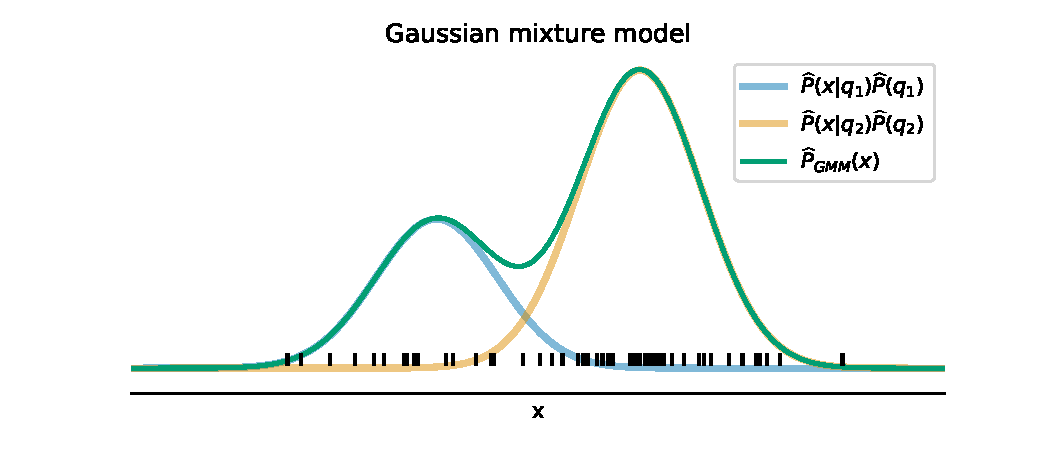
\includegraphics[width=0.7\textwidth]{img/latentexample_gmm}
	\notesonly{\captionof{figure}{A Gaussian Mixture Model as a latent variable model}}
\end{center}

``Groups'' may exist in the data. There are \emph{hidden causes} in the observations. We need a fit that accounts for this.

\end{frame}

\begin{frame}{Assignment variables as latent variables}

A simple way to understand what latent variables represent is to view them as assignment variables to components that we need to estimate.

Example:\\

\begin{itemize} 
\item assignment variables: $\vec{m}^{(\alpha)} =  \big( m_1^{(\alpha)}, \dots, m_M^{(\alpha)} \big)^\top \in \left\{ 0, 1 \right\}^M$ \\
		\begin{align}
		m_q^{(\alpha)} &= 
		\begin{cases}
		1, & \text{if component } q \text{ has generated point}~\alpha\\
		0, & \text{otherwise}
		\end{cases}
		%\hspace{0.5cm}
		\;\text{with} \;
		 \sum_{q=1}^{M} m_q^{(\alpha)} = 1 
		\end{align}
\end{itemize}

\end{frame}

\begin{frame}{Gaussian Mixture Models are latent variable models}

\slidesonly{
\begingroup
\small
\begin{itemize} 
\item assignment variables: $\vec{m}^{(\alpha)} =  \big( m_1^{(\alpha)}, \dots, m_M^{(\alpha)} \big)^\top \in \left\{ 0, 1 \right\}^M$ \\
		\begin{align}
		m_q^{(\alpha)} &= 
		\begin{cases}
		1, & \text{if component } q \text{ has generated point}~\alpha\\
		0, & \text{otherwise}
		\end{cases}
		%\hspace{0.5cm}
		\;\text{with} \;
		 \sum_{q=1}^{M} m_q^{(\alpha)} = 1 
		\end{align}
\end{itemize}
\endgroup
}

\notesonly{We have also seen how Gaussian Mixture Models can model assignment variables using mixture components.}

\begin{center}
	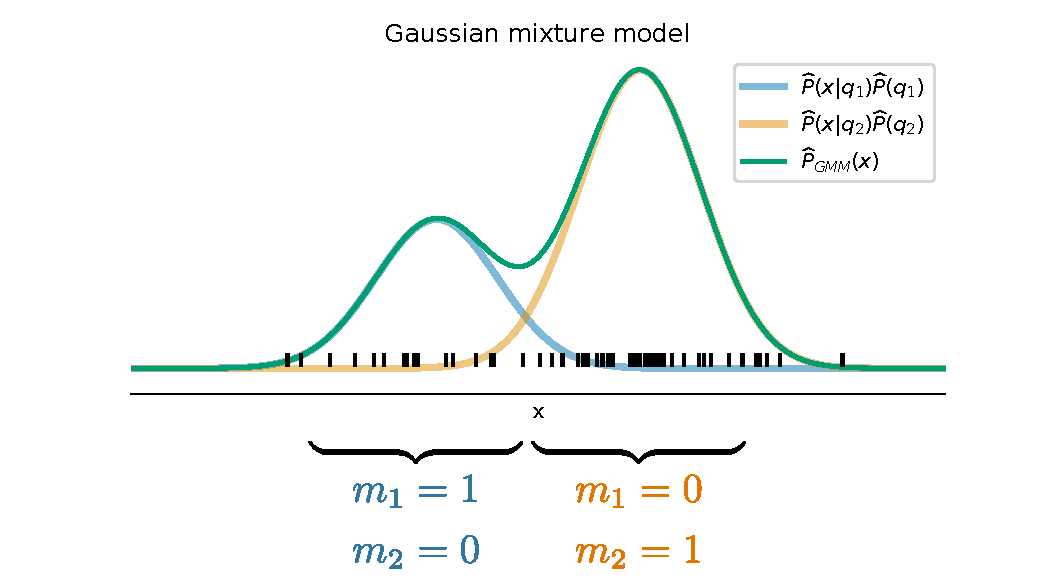
\includegraphics[width=0.7\textwidth]{img/latentexample_gmm_annot}
	\notesonly{\captionof{figure}{A Gaussian Mixture Model as a latent variable model with values of the assignment variables for the different groups in the data.}}
\end{center}


\end{frame}

\mode*

\mode<all>
\section{A latent variable model for temporal data}

%%%%%%%%%%%%%%%%%%%%%%%%%%%%%%%%%%%%%%%%%%%%%%%%%%%%%%%%%%%%%%%

\begin{frame}{Let's talk about the weather}

\svspace{-5mm}

\begin{center}
	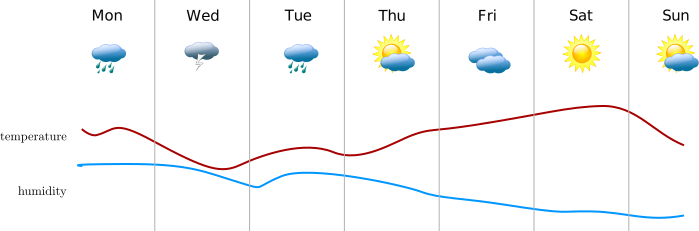
\includegraphics[width=0.7\textwidth]{img/weather}
\end{center}

\begin{center}
\slidesonly{
\only<2>{
	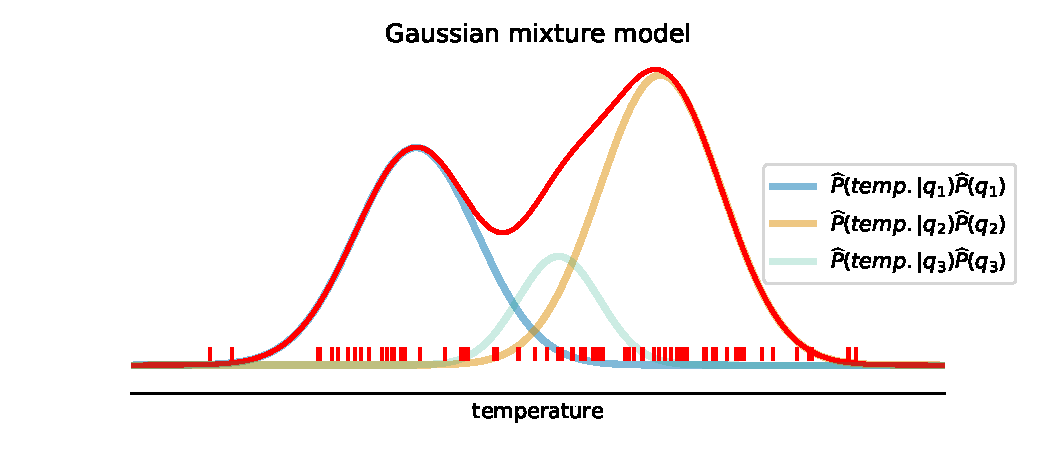
\includegraphics[width=0.6\textwidth]{img/latentexample_gmm_weather}
	}
}
\only<3>{
	\includegraphics<3>[width=0.6\textwidth]{img/latentexample_gmm_weather_icons}
}
	\notesonly{\captionof{figure}
	{Density estimation that does not account for any temporal aspects}
	}\slidesonly{\captionof*{figure}
	{Density estimation that does not account for any temporal aspects}
	}
\end{center}

\end{frame}

\begin{frame}{It's not all about amplitudes}

\begin{center}
	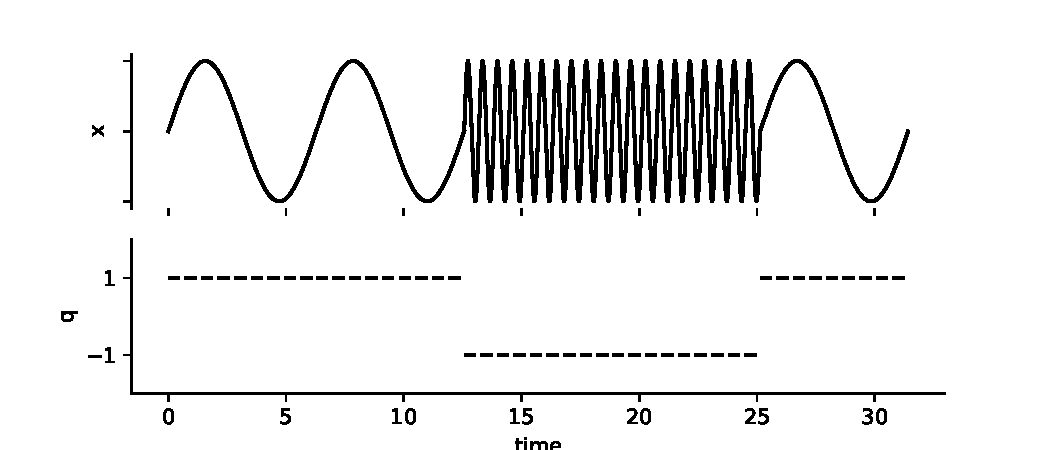
\includegraphics[width=0.9\textwidth]{img/sin}
\end{center}


\end{frame}

\begin{frame}

\begin{itemize}
\only<1->{
\item We have a sequence of observed events: $\vec x^{(t)} \in \R^N$
\item successive events $\vec x^{(t)}, \vec x^{(t-1)}$ \underline{cannot} be treated as independent
}
\slidesonly{
\svspace{10mm}
\only<2>{
\begin{minipage}{0.45\textwidth}
	\captionof*{figure}{at t=1}
	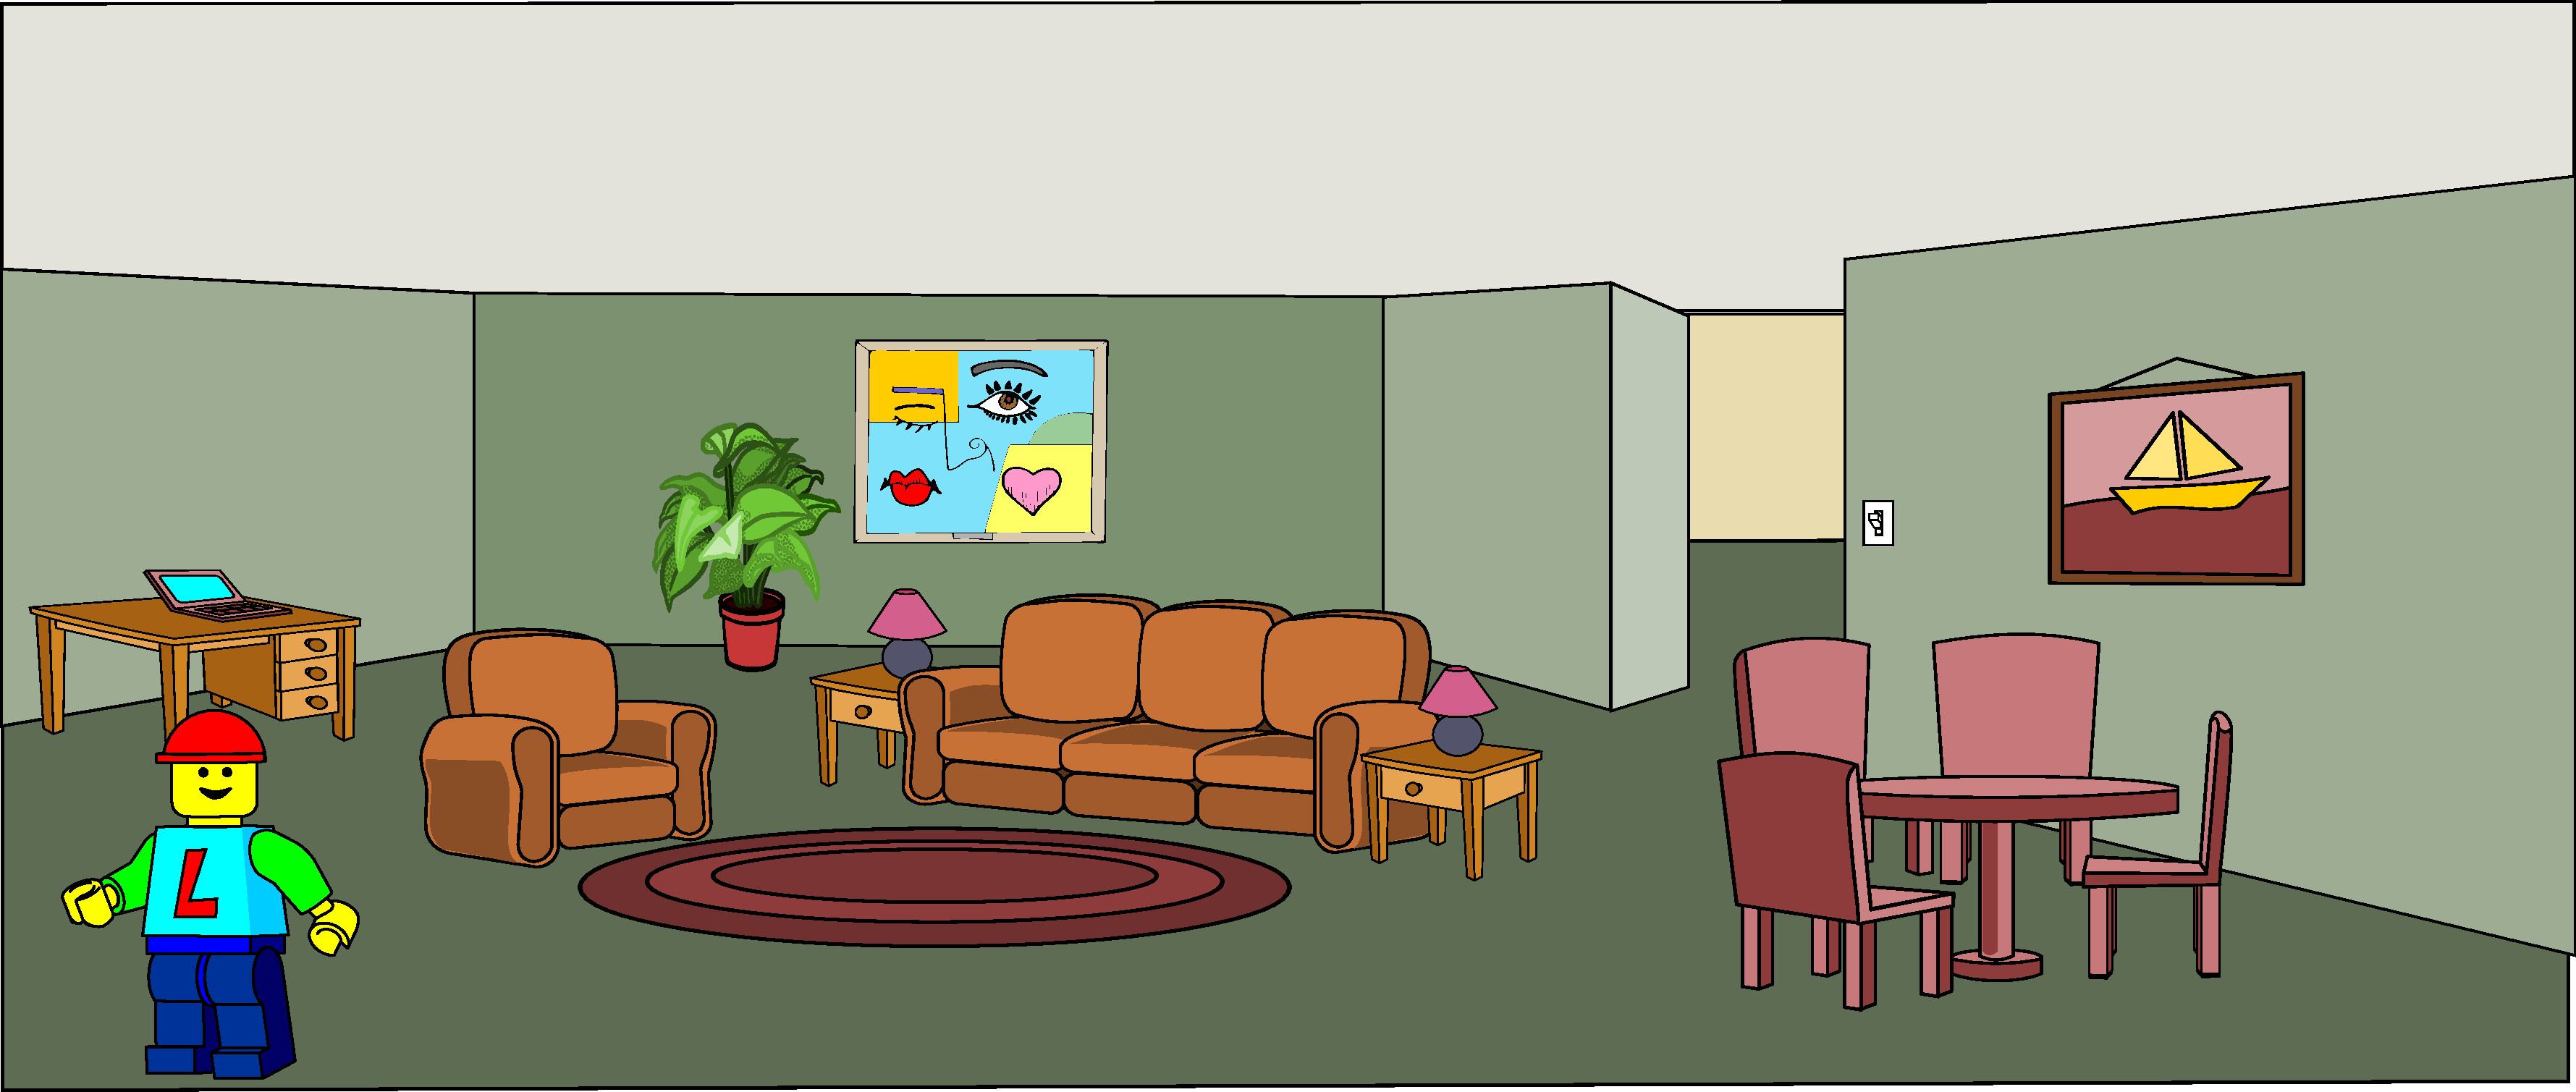
\includegraphics[width=0.99\textwidth]{img/Living-Room-Scene_001_figure_1}
\end{minipage}
\begin{minipage}{0.45\textwidth}
	\captionof*{figure}{at t=2}
	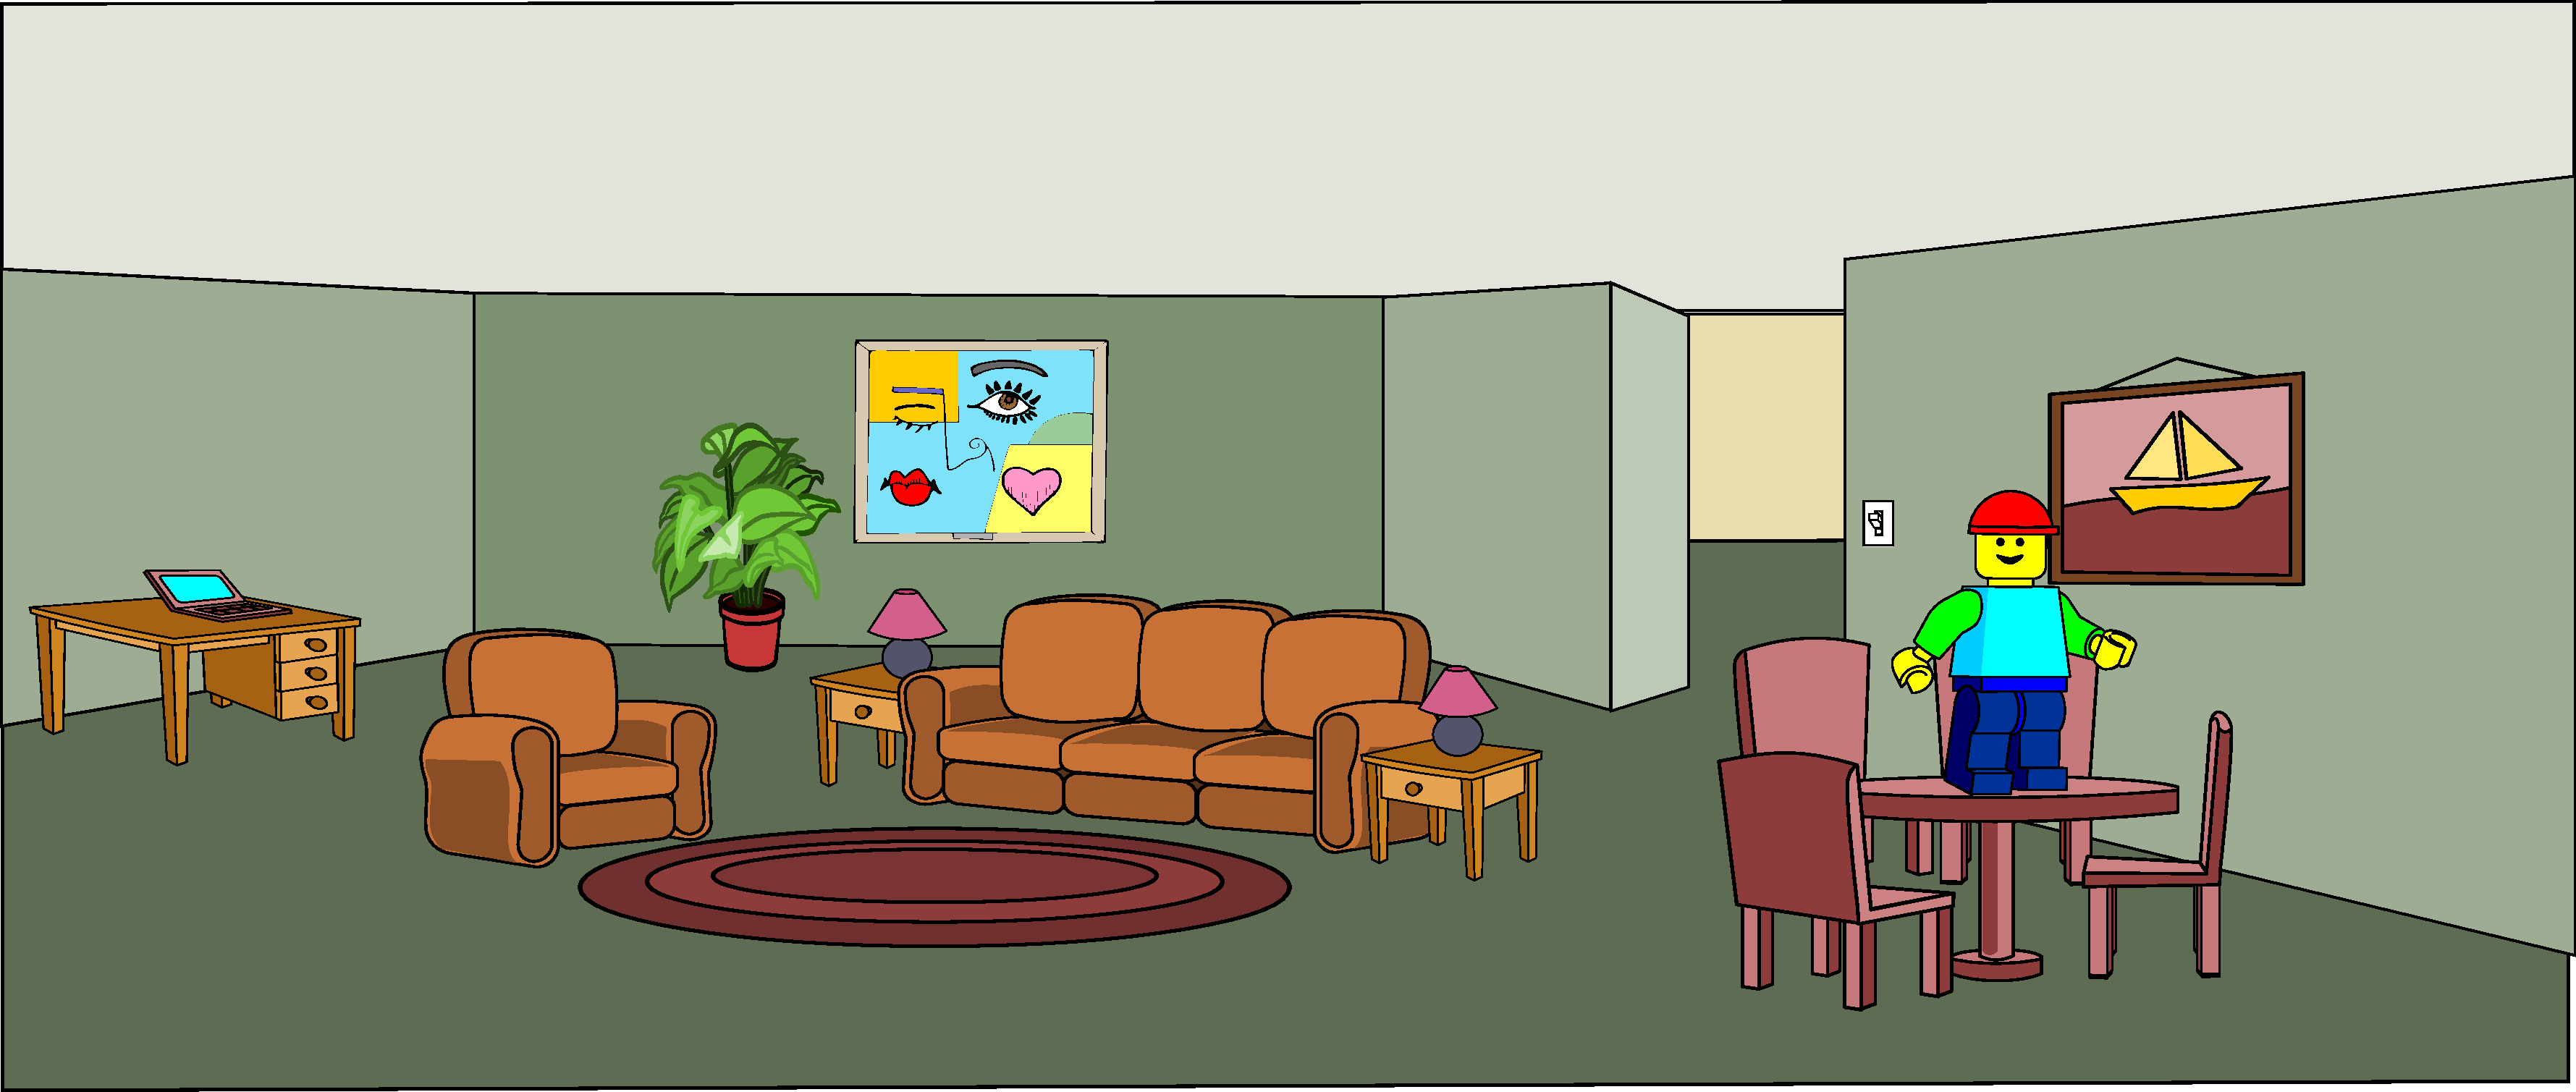
\includegraphics[width=0.99\textwidth]{img/Living-Room-Scene_001_figure_2}
\end{minipage}\\

\begin{minipage}{0.45\textwidth}
	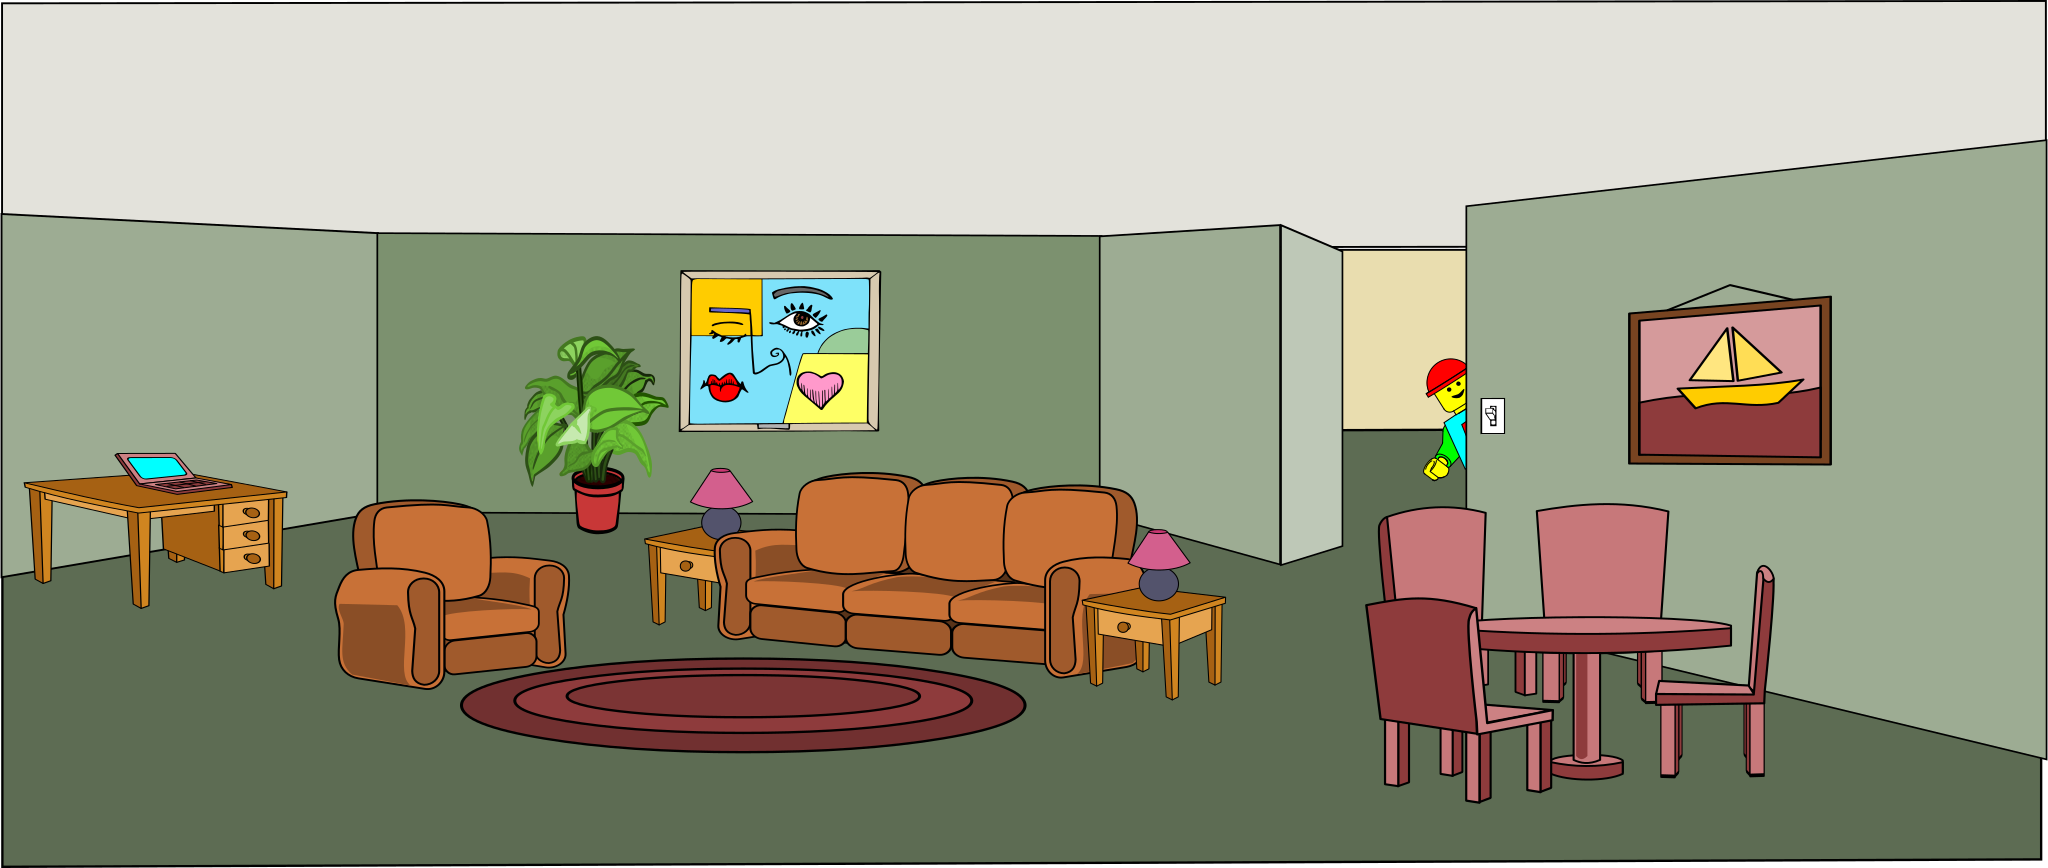
\includegraphics[width=0.99\textwidth]{img/Living-Room-Scene_001_figure_3}
	\captionof*{figure}{at t=3}
\end{minipage}
\begin{minipage}{0.45\textwidth}
	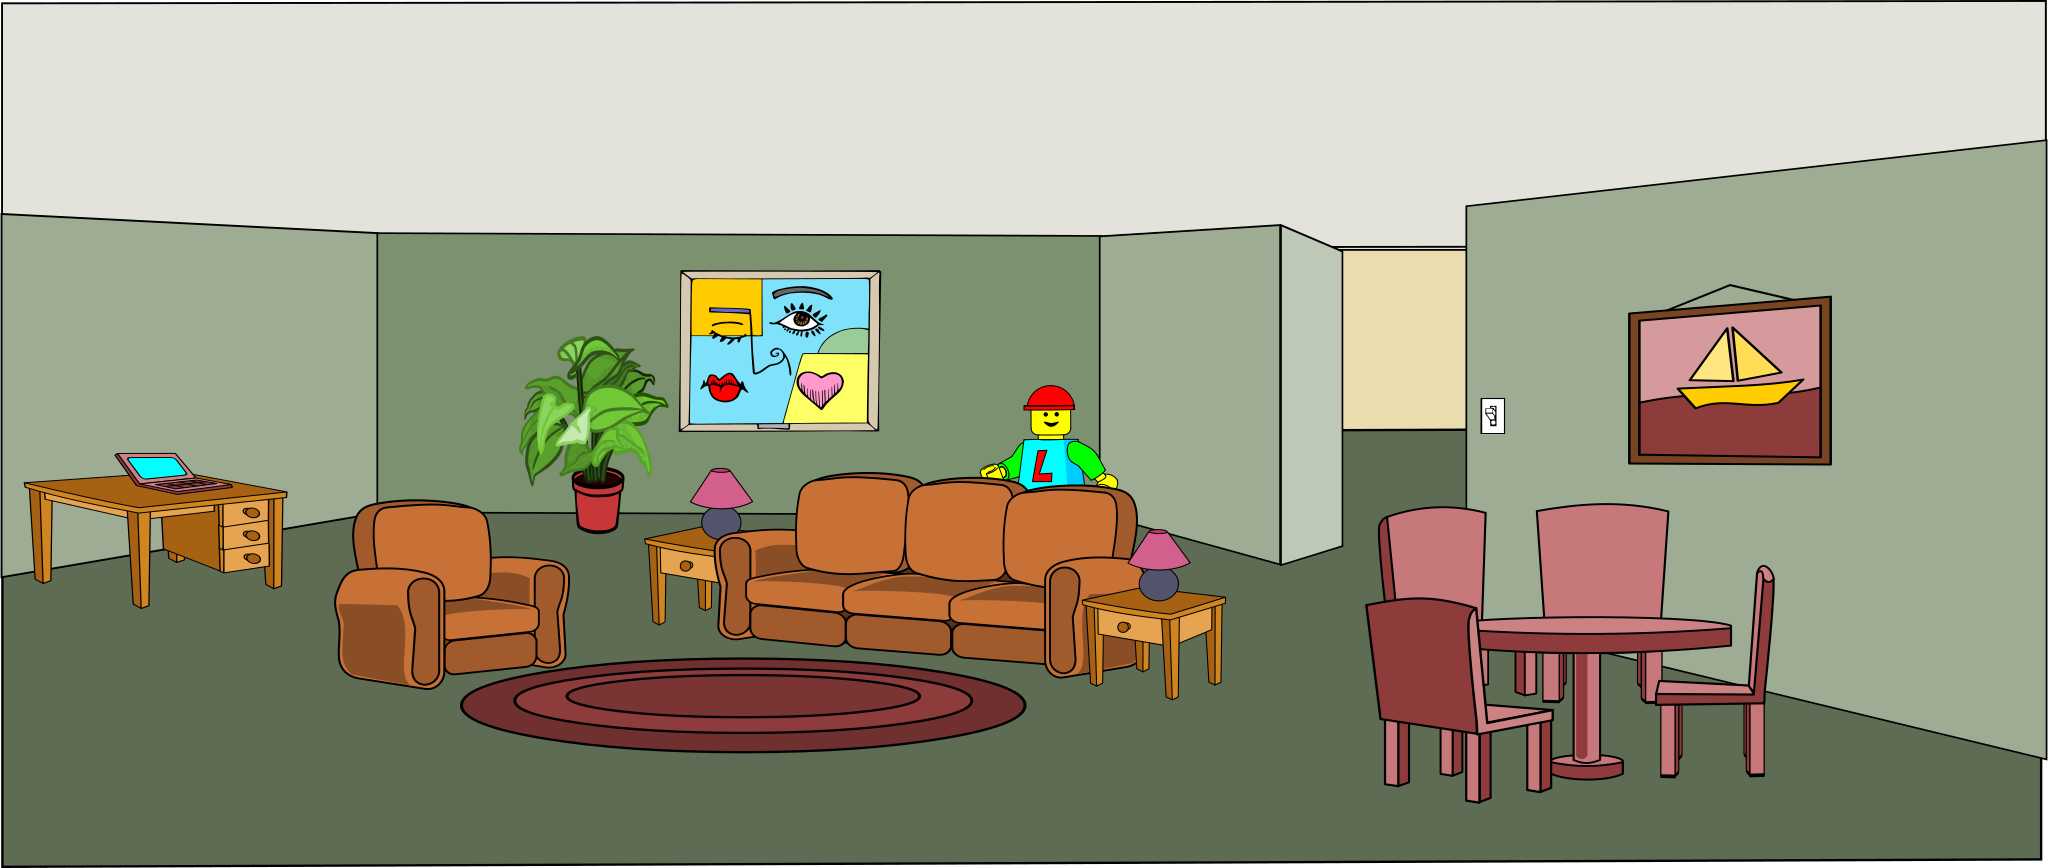
\includegraphics[width=0.99\textwidth]{img/Living-Room-Scene_001_figure_4}
	\captionof*{figure}{at t=4}
\end{minipage}
	}
}
\only<3->{
\item Assumption:\\
What we observe at every time step in the sequence $\{ \vec x^{t}\}_{t=1}^{T}$ is a result of the ``system'' being in a specific \emph{hidden state} at every time step $t$:\\
e.g. 1-out-of-$M$ coding for $M$ different states:
\begin{itemize} 
\item $\vec{m}^{(t)} = \big( m_1^{(t)}, \dots, m_M^{(t)} \big)^\top \in \left\{ 0, 1 \right\}^M$ \\
		\begin{align}
		m_q^{(t)} &= 
		\begin{cases}
		1, & \text{if system is in state } q \text{ at time}~t\\
		0, & \text{otherwise}
		\end{cases}
		%\hspace{0.5cm}
		\;\text{with} \;
		 \sum_{q=1}^{M} m_q^{(t)} = 1 
		\end{align}
\end{itemize}
\item Our observed sequence is a result of this \emph{hidden state} sequence
}
\end{itemize}

\end{frame}

\begin{frame}{Only}
\frametitle{Possibilities}

We may want to do:
\begin{itemize}
\item<only@1> Describe the sequence of hidden states:
$\{ \vec m^{(1)}, \ldots, \vec m^{(t)}, \ldots, \vec m^{(T)}\} = \{ \vec m^{(t)}\}_{t=1}^{T} \stackrel{\substack{\text{for}\\ \text{brevity}}}{=} \{ \vec m^{(t)}\}$
after observing the the sequence $\{\vec x^{(t)}\}$\\

\svspace{5mm}

\begin{center}
	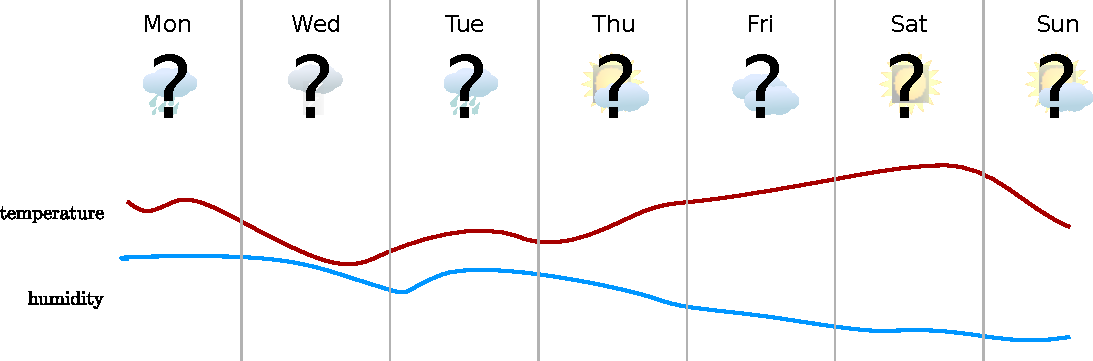
\includegraphics[width=0.7\textwidth]{img/weather_est_states}
	\notesonly{\captionof{figure}{Predict the sequence of hidden states}}
\end{center}

Example: hear sounds $\rightarrow$ what words were said? (transcribing speech)
\item<only@2> Generate a sequence of observations given a sequence of hidden variables $\{\vec m^{(t)}\}$
\\

\svspace{5mm}

\begin{center}
	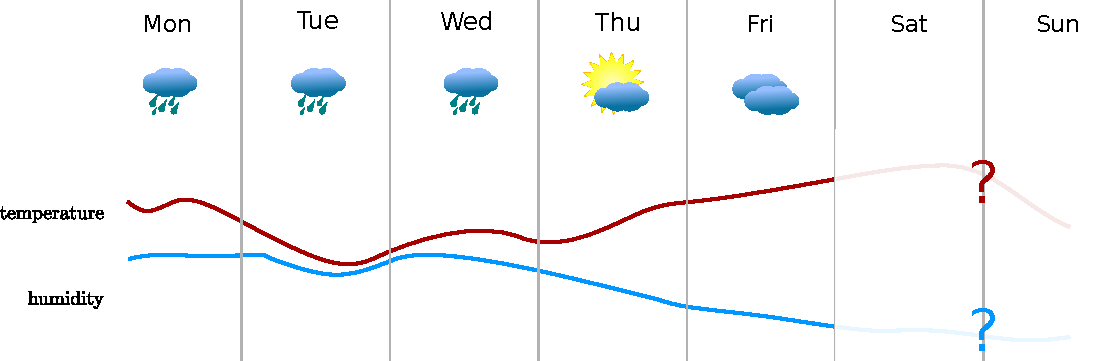
\includegraphics[width=0.7\textwidth]{img/weather_est_obs}
	\notesonly{\captionof{figure}{Predict the next sequence of observations}}
\end{center}

Example: type in words $\rightarrow$ hear speech (speech synthesis)
\item<only@3> Given a sequence $\{\vec x^{(t)}\}$ or $\{\vec m^{(t)}\}$ or both,\\
predict the next $\vec x$ and/or $\vec m$

\svspace{5mm}

\begin{center}
	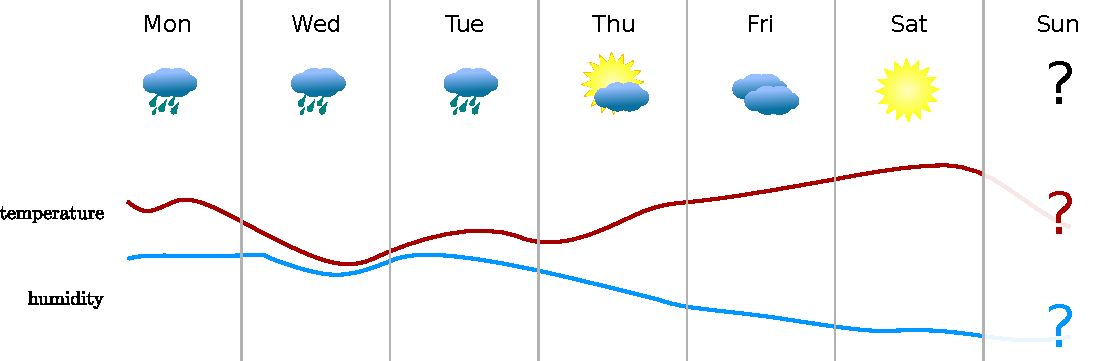
\includegraphics[width=0.7\textwidth]{img/weather_est_next}
	\notesonly{\captionof{figure}{Predict the next state and/or observation}}
\end{center}

\end{itemize}

\notesonly{
We can achieve all the above using Hidden Markov Models (HMM)
}

\end{frame}

\mode*

\clearpage

\mode<all>
\section{Markov chains}

\begin{frame} 
\mode<presentation>{
    \begin{center} \huge
        \secname
    \end{center}
    }
\mode<presentation>{
    \begin{center}
    Remember them from stochastic optimization?
    \end{center}
    }
\end{frame}

\begin{frame}{\secname}

Consider the random variables $y^{(1)}, y^{(2)}, \ldots, y^{(T-1)}, y^{(T)}$.
There is \textbf{no} statistical independence between the $y$'s:
\begin{equation}
P(y^{(1)}, y^{(2)}, \ldots, y^{(T-1)}, y^{(T)}) \ne \prod_{t=1}^T P(y^{(t)})
\end{equation}

But

\begin{equation}
P(y^{(t)} | y^{(t-1)}, y^{(t-2)}, \ldots, y^{(2)}, y^{(1)}) \ne P(y^{(t)} | y^{(t-1)})
\end{equation}

$y{(t)}$ depends only on $y^{(t-1)}$ $\rightarrow$ \emph{Markov property}

A sequence of samples of these $y$'s $\rightarrow$ \emph{Markov chain}

\end{frame}

\mode*

\clearpage

\mode<all>
\section{Hidden Markov Models (HMM)}

\begin{frame} 
\mode<presentation>{
    \begin{center} \huge
        \secname
    \end{center}
    }    
    \begin{center}
    Latent variable model for temporal data.
    \end{center}
	
\end{frame}

\begin{frame}{\secname}

HMMs operate on the following Markov chain of the latent variables:
\begin{equation}
P(\vec{m}^{(t)}  ~|~ \vec{m}^{(1)},  \dots,\vec{m}^{(t-1)}) =
		P(\vec{m}^{(t)}  ~|~ \vec{m}^{(t-1)})
\end{equation}

and that $\vec x^{(t)}$ depends directly on $\vec m^{(t)}$

\begin{equation}
P(\vec{x}^{(t)}  ~|~ \vec{x}^{(1)},  \dots,\vec{x}^{(t-1)}, \vec{m}^{(1)},  \dots,\vec{m}^{(t)}) =
		P(\vec{x}^{(t)}  ~|~ \vec{m}^{(t)})
\end{equation}

We want to estimate the above densities in the graphical model that is the HMM

\end{frame}

\begin{frame}{Recap: Latent variable models - the likelihood}

Latent variable models operate on the joint distribution of the observed and hidden variables.
The likelhood is recovered by \textcolor{blue}{marginalizing} the latent variable.
Recall in the general case of latent variable models:

\begin{equation}
P \left( \vec{x}^{(\alpha)} | \vec{w} \right) =
\kern-4ex
\underbrace{{\color{blue}\sum_{\vec{m}}}}_{
\substack{
\text{\tiny all possible}\\
\text{\tiny valid assignments}\\
\text{\tiny for point }\alpha}} 
\kern-3ex
P \left( \vec{x}^{(\alpha)}, \vec{m} | \vec{w} \right)
\end{equation}

\pause

\svspace{-5mm}

For HMMs\notesonly{ this would take the following shape}:

\svspace{-5mm}

\begin{equation}
P \left( \vec{x}^{(t)} |~\text{param.} \right) =
\kern-5ex
\underbrace{{\color{blue}\sum_{\vec{m}}}}_{
\substack{
\text{\tiny all possible}\\
\text{\tiny valid assignments}\\
\text{\tiny at step t}
}
}
\kern-3ex
P \left( \vec{x}^{(t)}, \vec{m}^{(t)} |~\text{param.} \right)
\stackrel{\substack{\text{for}\\
\text{brevity}}}{=}
{\color{blue}\sum_{\vec{m}}}
P \left( \vec{x}^{(t)}, \vec{m}^{(t)} \right)
\end{equation}

\pause

Next: Formulation of the joint distribution of the entire sequence

\pause

\question{What do we need this for?}

\notesonly{
-The optimization of the HMM boils down to maximizing the data likelihood. In this case the likelihood of the observed sequence. And for a latent variable model such as the HMM, this requires marginalization of the latent variables for all time steps in the sequence.
}

\end{frame}

\begin{frame}{The factorization corresponding to the graphical model of the HMM}

\notesonly{The factorization corresponding to the graphical model of the HMM:}

\slidesonly{
From the Markov property in the HMM:
\begin{equation}
P(\vec{m}^{(t)}  ~|~ \vec{m}^{(1)},  \dots,\vec{m}^{(t-1)}) =
		{\color{magenta}P(\vec{m}^{(t)}  ~|~ \vec{m}^{(t-1)})}
\end{equation}

and that $\vec x^{(t)}$ depends directly on $\vec m^{(t)}$

\begin{equation}
P(\vec{x}^{(t)}  ~|~ \vec{x}^{(1)},  \dots,\vec{x}^{(t-1)}, \vec{m}^{(1)},  \dots,\vec{m}^{(t)}) =
		{\color{cyan}P(\vec{x}^{(t)}  ~|~ \vec{m}^{(t)})}
\end{equation}
}

We exploit the markov property to factorize the joint distribution for the observed and hidden sequences.

\begin{align}
P(\{\vec{x}^{(t)}\}  , \{\vec{m}^{(t)}\}) = 
		P(\vec{m}^{(1)})
		\Bigg\lbrack
		\prod_{t=2}^T
		{\slidesonly{\color{magenta}}
		P(\vec{m}^{(t)} ~|~ \vec{m}^{(t-1)})
		}
		\Bigg\rbrack
		\prod_{t=1}^T 
		{\slidesonly{\color{cyan}}
		P(\vec{x}^{(t)} ~|~ \vec{m}^{(t)})
		}
\end{align}


\end{frame}

\subsection{Parameters of an HMM}

\definecolor{darkgreen}{rgb}{0,0.6,0}

\begin{frame}{\subsecname}

The parameters of an HMM are split into the following sets:
\begin{enumerate}
\item {Transition probabilities}:\\
The probability of going from state $q$ to $r$ \notesonly{(\sectionref{sec:hmm_transition})}
\item The initial distribution:\\
The probability of a state initiating a sequence.  \notesonly{(\sectionref{sec:hmm_init})}
\item Emission probabilities:\\
the distribution of observations given the hidden state $q$.  \notesonly{(\sectionref{sec:hmm_emission})}
\end{enumerate}

\end{frame}

\subsubsection{Transition model}
\label{sec:hmm_transition}

\begin{frame}{\subsubsecname}

{Transition probabilities}\only<1-4>{:\\
The probability of going from state $q$ to $r$:\\
\only<1>{
	\begin{equation}
	A_{qr}^{(t)} :=	P(m_r^{(t)} = 1 ~|~  m_q^{(t - 1)} = 1)
	\end{equation}
	\notesonly{Store all transition probabilities in a }transition probability matrix
	\begin{equation}
	\vec A^{(t)} \in \lbrack 0, 1\rbrack^{M\times M} \quad \text{(stochastic matrix)}
	\end{equation}
	with $\sum_{r=1}^M A_{qr}^{(t)} = 1 \quad \forall q= 1, \dots, M$\\
	Assuming homogeneity simplifies this by reducing the transitions to a single matrix $\vec A$ independent of time step t.
}
\only<1-4>{
	\begin{equation}
	P(\vec{m}^{(t)} ~|~ \vec{m}^{(t - 1)}, \vec{A}) = \prod_{r=1}^M \prod_{q=1}^M A_{qr}^{m_q^{(t-1)} m_r^{(t)}}
	\end{equation}
}
\only<2-4>{
\question{What is the probability of a sequence of states ``$3, 1, 2, 5$''?}

\only<3>{
	\svspace{-3mm}

	1-out-of-$M$ coding implies:
	\begin{itemize}
	\item[] state ``\textcolor{blue}{3}'': $\vec m = (0, 0, {\color{blue}1}, 0, \ldots, 0)^\top$,
	\item[] state ``\textcolor{darkgreen}1'': $\vec m = ({\color{darkgreen}1}, 0, 0, 0, \ldots, 0)^\top$
	\end{itemize}

	\begingroup
	\small
	\begin{align}
		P(\text{``}3, 1, 2, 5\text{''} | \vec A) 
		&= A_{31} \cdot A_{12} \cdot A_{25} \\
		&\kern-7ex= 
		%{\tiny 
		P(\vec{m}^{(2)} ~|~ \vec{m}^{({1})}, \vec{A}) \cdot P(\vec{m}^{(3)} ~|~ \vec{m}^{(2)}, \vec{A}) \cdot P(\vec{m}^{(4)} ~|~ \vec{m}^{(3)}, \vec{A})
	\end{align}
	\endgroup
}

\only<4>{
	The probability of a sequence $\{\vec m^{(t)}\}$ in general:

	\begingroup
	\small
	\begin{align}
		P(\{\vec m^{(t)}\} | \vec A) = \prod_{t={\color{red}2}}^{T} P(\vec{m}^{(t)} ~|~ \vec{m}^{({\color{red}t - 1})}, \vec{A})
	\end{align}
	\endgroup
	}
}
}

\end{frame}

\subsubsection{Initial distributions}
\label{sec:hmm_init}


\begin{frame}{\subsubsecname}

Initial distributions (considered part of the transition model):\\
The probability of the initial state is given by the distribution
\begin{equation}
P(\vec{m}^{(1)} ~|~ \vec{b}) = \prod_{q=1}^M b_q^{m_q^{(1)}}
\end{equation}
	parameterized by probability vector $\vec{b} \in [0, 1]^M$ 
	
	whose elements $b_q := P(m_q^{(1)} = 1)$ satisfy $\sum_{q=1}^M b_q = 1$

	($\leadsto ~ \vec{b}$ has $M-1$ degrees of freedom)
	
	\pause
	
	Example from text data:\\
	\begin{equation}
		P(\text{``}\text{Once upon a time}\text{''}) > P(\text{``}\text{lived happily ever after}\text{''})
	\end{equation}
	
	\svspace{5mm}
	
	$\leadsto$ transition model $\vec{m}^{(1)}$ and $\vec{m}^{(t-1)} \rightarrow \vec{m}^{(t)}$ for $t=2, \dots, T$
	
	\hspace{5mm} fully specified through parameters $\vec{A}$ and $\vec{b}$

\end{frame}


\subsubsection{Emission model}
\label{sec:hmm_emission}


\begin{frame}{\subsubsecname}

Emission probabilities $P(\vec x^{(t)} | \vec m^{(t)} ; \vec \phi)$

Where $\vec \phi = \{\vec \phi_1, \ldots, \vec \phi_M\}$ specifies the parameters of the set of $M$ components.

Analogous to mixture components $P(\vec x| q)$ of a mixture model, e.g. choosing Gaussian basis functions
\begin{equation}
P(\vec{x} ~|~ \vec{m}, \vec{\boldsymbol{\phi}}) = \prod_{q=1}^M
	P(\vec{x}^{(t)} ~|~ \vec{\boldsymbol{\phi}}_q)^{m_q^{(t)}} := \prod_{q=1}^M \mathcal{N}^{m_q} (\vec{x} ~|~ \vec{\boldsymbol{\mu}}_q, \vec{\Sigma}_q)
\end{equation}
				
where $\vec{\boldsymbol{\phi}} := \big\{\underbrace{\vec{\boldsymbol{\mu}}_q, \vec{\Sigma}_q}_{\vec{\boldsymbol{\phi}}_q} \big\}_{q=1}^M$

Example:\\
\begin{equation}
P(\mathit{temperature}=29^{\circ}, \mathit{humidity}=20\% | \text{``}\mathit{cloudy}\text{''}; \vec \phi)
\end{equation}

\end{frame}

%%%%%%%%%%%%%%%%%%%%%%%%%%%%%%%%%%%%%%%%%%%%%%%%%%%%%%%%%%%%%%%%%%%%%%
\begin{frame}{The parametrized HMM}
	
A more detailed specification of the joint distribution becomes:
	
	\begin{align}
	&P(\{\vec{x}^{(t)}\}  , \{\vec{m}^{(t)}\} ~|~ \vec{w})
	 \\&
	~=P(\vec{m}^{(1)})
	\Bigg\lbrack
	\prod_{t=2}^T
	P(\vec{m}^{(t)} ~|~ \vec{m}^{(t-1)})
	\Bigg\rbrack
	\prod_{t=1}^T P(\vec{x}^{(t)} ~|~ \vec{m}^{(t)})
	\\&~=
	\underbrace{P(\vec{m}^{(1)}~|~ \vec{b})}_{\text{initial hidden state}}
	\prod_{t=2}^{T} 
		\underbrace{P(\vec{m}^{(t)}~|~  \vec{m}^{(t - 1)},~ \vec{A})
		}_{\text{transition to next hidden state}}
	\prod_{t=1}^{T} 
	\underbrace{P(\vec{x}^{(t)}~|~  \vec{m}^{(t)},~ \vec{\boldsymbol{\phi}})
	}_{\text{emission model $\leadsto$ observation}}
	\end{align}
	
	where $\vec{w} := \{ 
	\kern-3.5ex
		\underbrace{\vec{A}}_{\substack{\text{state transition} \\ \text{probabilities}}}, \underbrace{\vec{b}}_{\substack{\text{initial state} \\ \text{probabilities}}}, \underbrace{\vec{\boldsymbol{\phi}}}_{\substack{\text{emission} \\ \text{components}}} 
	\kern-2.5ex
		\}$ summarizes the model parameters
	
\end{frame}
%%%%%%%%%%%%%%%%%%%%%%%%%%%%%%%%%%%%%%%%%%%%%%%%%%%%%%%%%%%%%%%%%%%%%%

\mode*

\mode<all>
\section{Inference in HMMs: the forward-backward algorithm}

\begin{frame} 
\mode<presentation>{
    \begin{center} \huge
        \secname
    \end{center}
    }    
    \begin{center}
    What can we do with a \underline{trained} HMM model
    \end{center}
	
\end{frame}

\begin{frame}

\begin{itemize}
\item[] \textbf{Goal}: Compute the probability of a state at any step $t$ given the observed sequence:
\begin{equation}
P(\vec{m}^{(t)}  ~|~ \vec{x}^{(1)},  \ldots,\vec{x}^{(T)}) =
		P(\vec{m}^{(t)}  ~|~ \{\vec{x}^{(t-1)}\})
\end{equation}

\item[] \textbf{Assumptions}: parameters $\vec{w} := \{
		\vec{A}
		\vec{b}
		\vec{\boldsymbol{\phi}}
		\}$ are \underline{known} (have been found) We will cover estimating these parameters later.
\item[] \textbf{Procedure}: The forward-backward algorithm yields an expression for $P(\vec{m}^{(t)}  ~|~ \{\vec{x}^{(t-1)}\})$

\end{itemize}

\end{frame}

\subsection{The Forward algorithm}

\begin{frame}{\subsecname}

The Forward algorithm computes the joint distribution $P(\vec x^{(1)}, \ldots , \vec x^{(t)}, \vec m^{(t)}) \stackrel{\substack{\text{for}\\ \text{brevity}}}{=} P(\{\vec x^{(s)}\}_{s=1}^t, \vec m^{(t)})$\\
for any step $t \in \lbrack 1, T\rbrack$.\\

\svspace{5mm}

Here, $\{\vec x^{(s)}\}_{s=1}^t$ denotes the sequence of observations leading up to step $t$\\

\svspace{5mm}

Example intepretation for $P(\{\vec x^{(s)}\}_{s=1}^t, \vec m^{(t)})$: ``The distribution of temperature and humidity measures that lead up to a ``sunny'' day on day $t$.''

\end{frame}

\begin{frame}{\subsecname}

The joint distribution $P(\{\vec x^{(s)}\}_{s=1}^t, \vec m^{(t)})$ for any step $t \in \lbrack 1, T\rbrack$ is computed by \textit{marginalizing over the previous step in order to move ``forward''}:

\begin{equation}
P(\{\vec x^{(s)}\}_{s=1}^t, \vec m^{(t)})
=
\kern-3ex
\underbrace{
\sum_{\vec m^{(t-1)}}
}_{
\substack{
\text{\tiny all possible}\\
\text{\tiny valid assignments}\\
\text{\tiny at the previous}\\
\text{\tiny step t-1}
}
}
\kern-3ex
P(\{\vec x^{(s)}\}_{s=1}^t, \vec m^{(t)}, \vec m^{(t-1)})
\end{equation}

\end{frame}

\begin{frame}{\subsecname}
%\svspace{-5mm}

\begin{align}
\slidesonly{
\only<1->{
	P(\{\vec x^{(s)}\}_{s=1}^t, \vec m^{(t)})
}
\only<1,2>{
	&=
	\sum_{\vec m^{(t-1)}}
	P(\{\vec x^{(s)}\}_{s=1}^t, \vec m^{(t)}, \vec m^{(t-1)})
}
}
\only<1,2>{
	\intertext{Applying the product rule:}
	&=
	\sum_{\vec m^{(t-1)}}
	\bigg\lbrack
	P(\vec x^{(t)}~|~\{\vec x^{(s)}\}_{s=1}^{t-1}, \vec m^{(t)}, \vec m^{(t-1)})\\
	&\qquad\qquad\cdot 
	P(\vec m^{(t)}~|~\{\vec x^{(s)}\}_{s=1}^{t-1}, \vec m^{(t-1)})\\
	&\qquad\qquad\cdot 
	P(\vec m^{(t-1)},\{\vec x^{(s)}\}_{s=1}^{t-1})
	\bigg\rbrack
	}
\only<2>{
	\intertext{due to the Markov property
	$P(\vec x^{(t)}~|~\{\vec x^{(s)}\}_{s=1}^{t-1}, \vec m^{(t)}, \vec m^{(t-1)})
	=
	P(\vec x^{(t)}~|~\vec m^{(t)})
	$}\\
}
\only<3>{
	&=
	\sum_{\vec m^{(t-1)}}
	\bigg\lbrack
	P(\vec x^{(t)}~|~ \vec m^{(t)})\\
	&\qquad\qquad\cdot 
	P(\vec m^{(t)}~|~\{\vec x^{(s)}\}_{s=1}^{t-1}, \vec m^{(t-1)})\\
	&\qquad\qquad\cdot 
	\underbrace{
	P(\vec m^{(t{\color{red}-1})}, \{\vec x^{(s)}\}_{s=1}^{t{\color{red}-1}})
	}_{\text{recursion}}
	\bigg\rbrack
}
\end{align}


\only<3>{

To illustrate the recursion:

\begingroup
\footnotesize
\begin{align}
	P(&\{\vec x^{(s)}\}_{s=1}^{t{\color{red}-1}}, \vec m^{(t{\color{red}-1})})\\
	=&
	\kern-2ex
	\sum_{\vec m^{(t-1{\color{red}-1})}}
	\kern-1ex
	\bigg\lbrack
	P(\vec x^{(t{\color{red}-1})}|\vec m^{(t{\color{red}-1})})
	%\\
	%&\qquad\qquad
	%\cdot 
	P(\vec m^{(t{\color{red}-1})}|\{\vec x^{(s)}\}_{s=1}^{t-1{\color{red}-1}}, \vec m^{(t-1{\color{red}-1})})
	%\\
	%&\qquad\qquad
	%\cdot 
	\underbrace{
	P(\vec m^{(t{\color{red}-1}{\color{cyan}-1})}|\{\vec x^{(s)}\}_{s=1}^{t{\color{red}-1}{\color{cyan}-1}})
	}_{\text{recursion}}
	\bigg\rbrack
\end{align}
\endgroup
}

\end{frame}


\subsection{The Backward algorithm}

\begin{frame}{\subsecname}

The Forward algorithm computes the conditional distribution
$
P(
\underbrace{\vec x^{(t+1)}, \ldots, \vec x^{(T)}
}_{
\{\vec x^{(s)}\}_{s=t+1}^T
} | \vec m^{(t)})
$\\
for any step $t \in \lbrack0, T)$

Intepretation of the above distribution:\\

The distribution for the sub-sequence of observations \emph{following} step $t$

\slidesonly{No need to manipulate this further}

\end{frame}

\subsection{Forward-Backward}

\begin{frame}
\end{frame}

\mode*

\mode<all>
\subsection{Applying the forward-backward procedure}

\begin{frame} 
\mode<presentation>{
    \begin{center} \huge
        \subsecname
    \end{center}
    
    

\begin{equation}
P(\vec m^{(t)} | \{\vec x^{(s)}\}_{s=1}^T )
\frac{
{\color{orange}
P( \vec x^{(t+1)}, \ldots, \vec x^{(T)} | \vec m^{(t)} )
}
\cdot 
{\color{blue}
P(\vec m^{(t)}, \vec x^{(1)}, \ldots, \vec x^{(t)}) 
}
}{
P(\vec x^{(1)}, \ldots, \vec x^{(T)})
}
\end{equation}
    }
\end{frame}

\subsubsection{Inference}

\begin{frame}{\subsecname:~\subsubsecname}

Inference using the conditional distribution
$
P(\vec m^{(t)} | \{\vec x^{(s)}\}_{s=1}^T )
$

Example: ``Change detection''

\begin{equation}
P(\vec m^{(t)} \ne \vec m^{(t-1)} | \{\vec x^{(s)}\}_{s=1}^T )
\end{equation}

\svspace{5mm}

\slidesonly{
\begin{center}
	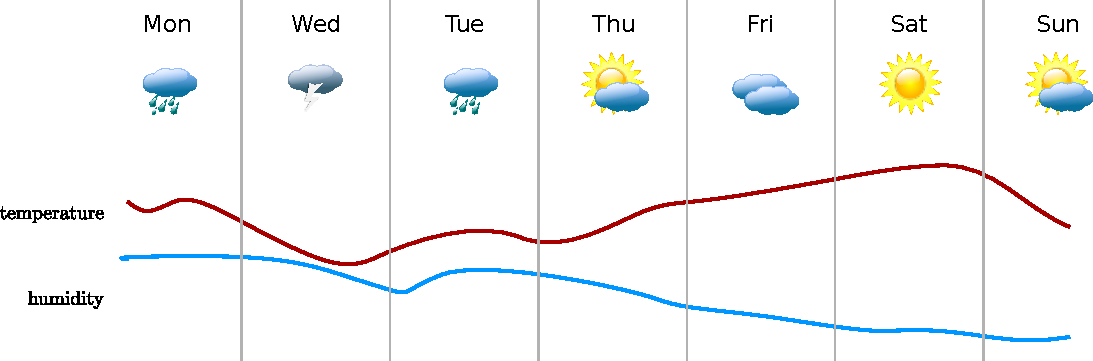
\includegraphics[width=0.6\textwidth]{img/weather_changedetection}
	\captionof*{figure}{What are the chances of two sunny days in a row?}
\end{center}
}

\end{frame}

\subsubsection{Parameter estimation}

\begin{frame}{\subsecname:~\subsubsecname}

Estimate the parameters $\vec{w} := \{
		\vec{A},
		\vec{b},
		\vec{\boldsymbol{\phi}}
		\}$ of an HMM.\\
		
The forward-backward procedure needs the parameters to be known but they need not necessarily be optimal.

\pause

\slidesonly{
\begin{center}
	
\includegraphics[width=0.3\textwidth]{img/meme_fwdbwdwork}
\end{center}
}

\end{frame}

\begin{frame}{\subsecname:~\subsubsecname}

\question{How do we estimate the parameters of an HMM?}

\pause

-Combine the forward-backward procedure with Expectation Maximization

\slidesonly{
\begin{center}
	
\includegraphics[width=0.5\textwidth]{img/meme_fwdbwdemintro}
\end{center}
}

\end{frame}

\begin{frame}{\subsubsecname}

\begin{block}{Baum-Welch Algorithm}
\begin{enumerate}
\item The forward-backward procedure is given intermediate estimates of the parameters to compute the distributions
\item The EM algorithm updates the parameters to maximize the likelihood of the data.
\end{enumerate}
\end{block}

\end{frame}

\subsubsection{Sampling from the posterior}

\begin{frame}{Only}
\frametitle{\subsecname:~\subsubsecname}

The forward-backward procedure can be applied to sample from the posterior
$
P(\{\vec m^{(t)} \} | \{\vec x^{(t)}\} )
$

\begin{itemize}
\item<only@1>
Example from speech recognition where
\begin{itemize}
\item $\{\vec m^{(t)} \}$ represents the sequence of phonemes,
\item $\{\vec x^{(t)} \}$ samples from audio file with speech.
\end{itemize}

\begin{center}
	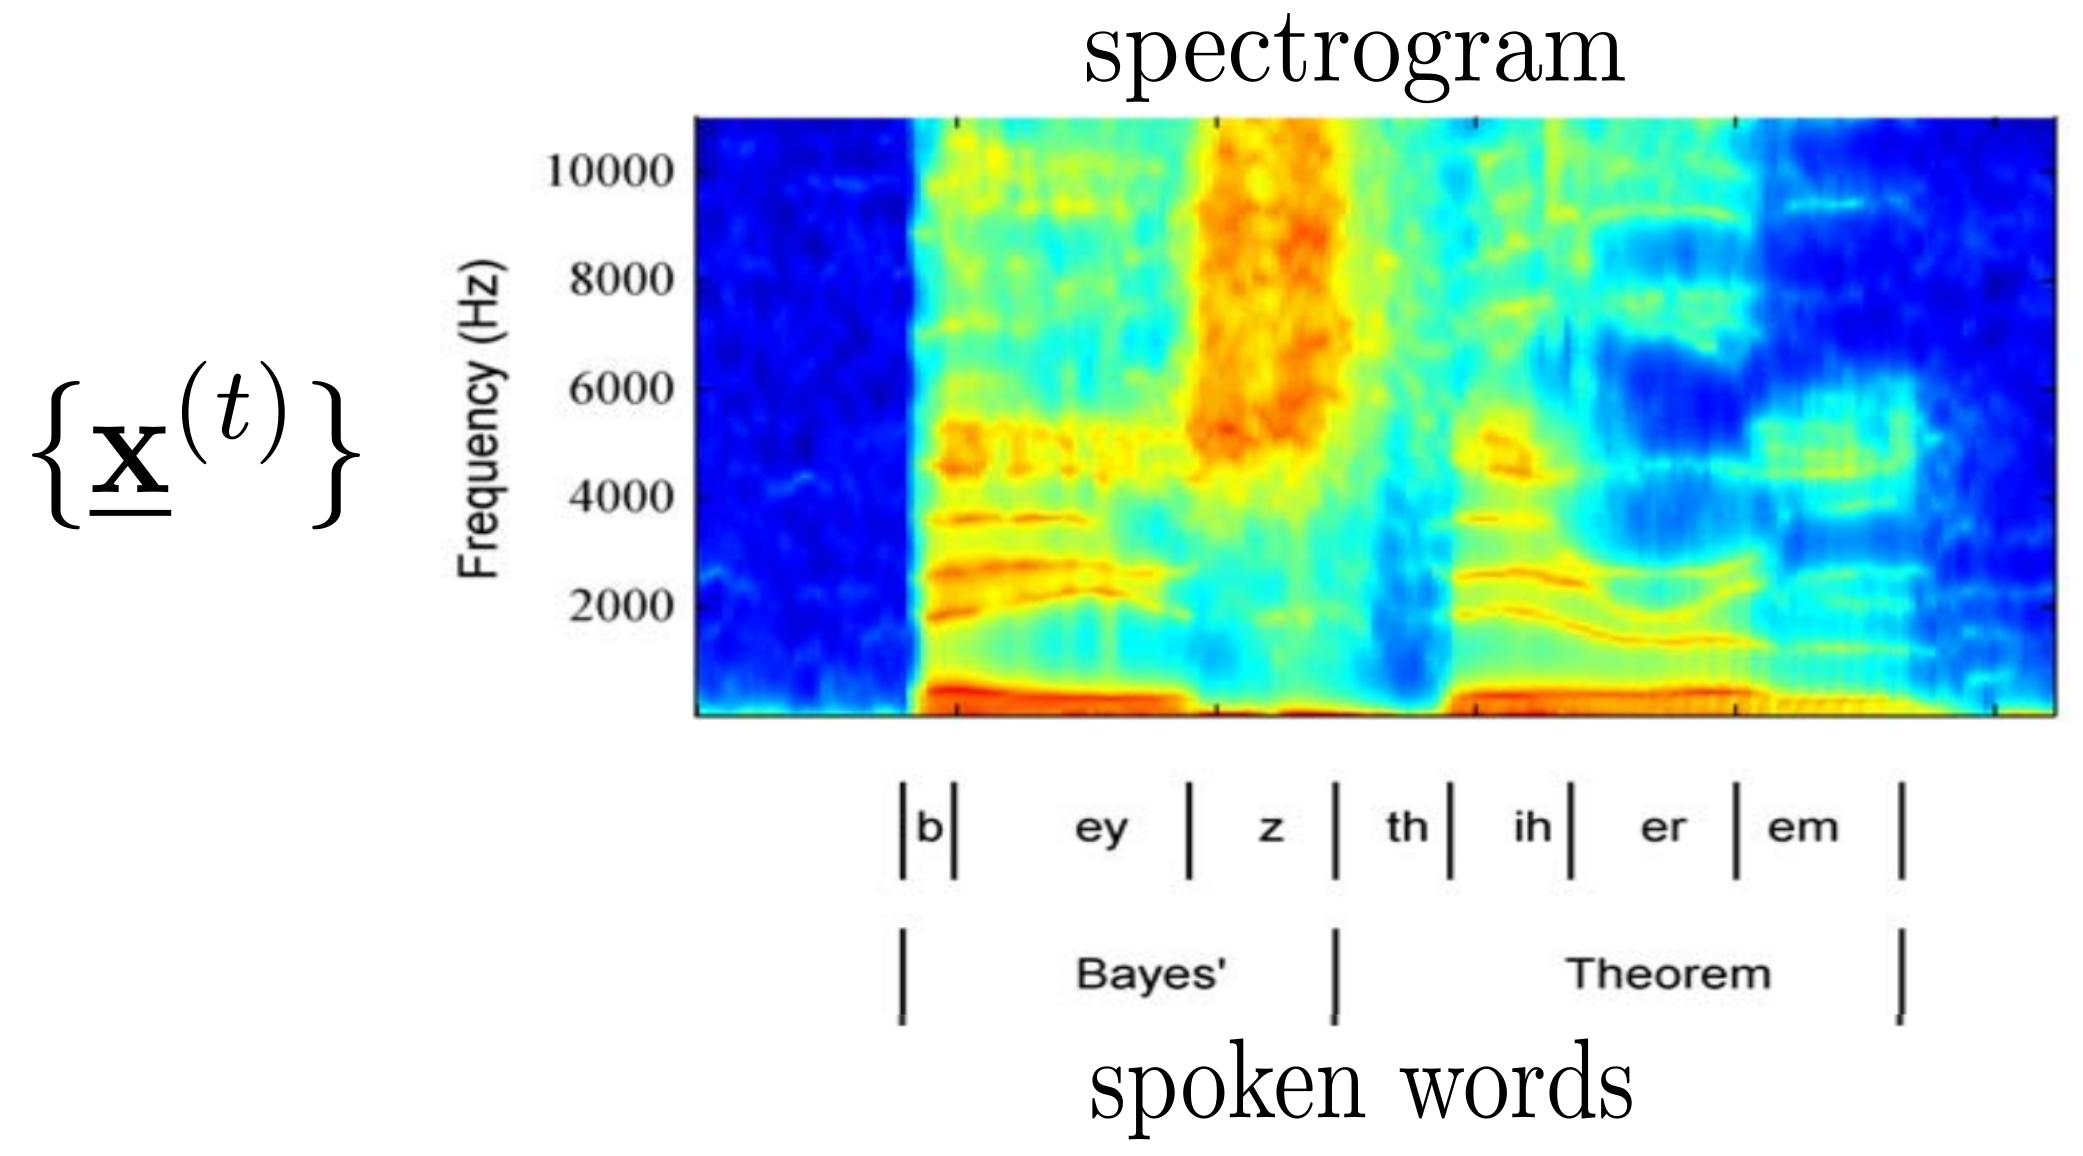
\includegraphics[width=0.6\textwidth]{img/Bishop_13-1}
	\slidesonly{\captionof*{figure}{Source: \citep{bishop2006pattern}}}
	\notesonly{\captionof{figure}{Source: \citep{bishop2006pattern}}}
\end{center}

\item<only@2> If we are interested in in the \emph{most likely} sequence, we employ the \emph{Viterbi algorithm}
to find:
\begin{equation}
\{\vec m_*^{(t)} \} = 
\argmax_{\{\vec m^{(t)} \}} P(\{\vec m^{(t)} \} | \{\vec x^{(t)}\} )
\end{equation}

\item<only@3>
If the dimensionality of $\vec m$ is much lower than $\vec x$ (e.g. 2-D vs. $N$-dim), we can sample from the posterior to visualize the sequence.

\end{itemize}

\end{frame}

\subsubsection{One-step-ahead prediction}

\begin{frame}{\subsecname:~\subsubsecname}

One-step-ahead prediction involves the conditional distribution:
\begin{align}
P(&\vec{x}^{(t+1)} ~|~ \vec{x}^{(1)}, \ldots, \vec{x}^{(t)}) 
= \\
&\sum_{\{\vec{m}^{(t+1)}, \vec{m}^{(t)} \}} P(\vec{x}^{(t+1)} | \vec{m}^{(t+1)}) \cdot P(\vec{m}^{(t+1)} | \vec{m}^{(t)}) \cdot~{\only<2>{\color{blue}}P(\vec{m}^{(t)} | \vec{x}^{(1)}, \ldots, \vec{x}^{(t)})}\\
\only<2>{
=& 
\sum_{\{\vec{m}^{(t+1)}, \vec{m}^{(t)} \}} 
\kern-2ex
P_{\mathit{emission}} \cdot P_{\mathit{tansition}} \cdot~{\color{blue}P(\mathit{the ~state~we~have~reached~so~far})}
}
\end{align}

\pause 

This only involves ${\color{blue}
P(\vec m^{(t)}, \vec x^{(1)}, \ldots, \vec x^{(t)}) 
}$ from the forward pass in addition to summing over the possible combinations of $\vec m^{(t)}$ and $\vec m^{(t+1)}$

\end{frame}

\mode*

%\clearpage

\section{References}
\begin{frame}[allowframebreaks] \frametitle{References}
	\scriptsize
	\bibliographystyle{plainnat}
	\bibliography{bibliography}
\end{frame}

\end{rightcolumn}
\end{paracol}

\end{document}
